\documentclass[cal1spr16Lectures.tex]{subfiles}
%\AtBeginSubsection{
%	\begin{frame}[allowframebreaks]{}
%	\begin{multicols}{2}
%	\tableofcontents[currentsubsection]
%	\end{multicols}
%	\end{frame}
%	}
	
\begin{document}

%\section[Week 6]{Week 6: 22-26 February}

% % %
\subsubsection{\bf Monday 22 February}
\begin{frame}[allowframebreaks]{Mon 22 Feb}
\begin{itemize}\footnotesize
\item Exam 1 Feedback

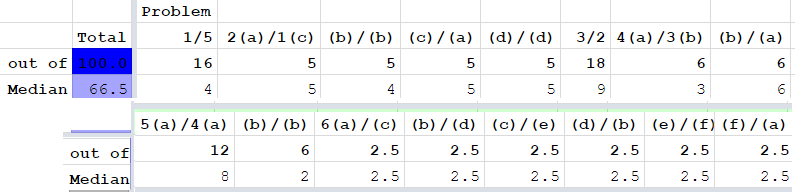
\includegraphics[scale=0.45]{../Exams/Exam1Medians}
\begin{center}
\includegraphics[scale=0.45]{../Exams/Exam1Spread}
\end{center}
\framebreak
\item MIDTERM 
\begin{itemize}
	\item Tuesday 8 March 6-7:30p
	\item If you have legitimate conflict, i.e., anything that is also scheduled in ISIS, I need to know now.  If you are not sure if it conflicts with a course, please have that instructor contact me ASAP.
	\item Cumulative.  Covers up to \S 3.9
	\item Morning Section: Walker rm 124
	
	Afternoon Section: Walker rm 218
\end{itemize}
\item Sub on Friday 26 Feb and Monday 29 Feb.
\item Exam 2: Friday 4 March.  Covers up to \S 3.8.
\end{itemize}
\end{frame}

% % %
\begin{frame}{}
The Quotient Rule also allows us to extend the Power Rule to negative numbers -- if $n$ is any integer, then 
\[\frac{d}{dx}\left[ x^n \right] = nx^{n-1}.\]
\begin{que} How? \end{que}
\end{frame}

% % %
\begin{frame}
\begin{exe} If $f(x)=\frac{x(3-x)}{2x^2}$, find $f^{\prime}(x).$ \end{exe}
\end{frame}

% % %
\subsubsection{Derivative of $e^{kx}$}
% % %

% % %
\begin{frame}{\small Derivative of $e^{kx}$}
For any real number $k$,
\[\frac{d}{dx} \left( e^{kx} \right) = ke^{kx}.\]
\begin{exe}What is the derivative of $x^2 e^{3x}$? \end{exe}
\end{frame}

% % %
\subsubsection{Rates of Change}
% % %

% % %
\begin{frame}{\small Rates of Change}\footnotesize
The derivative provides information about the instantaneous rate of change of the function being differentiated (compare to the limit of the slopes of the secant lines from \S 2.1).

\vspace{1pc}
For example, suppose that the population of a culture can be modeled by the function $p(t)$.  We can find the instantaneous growth rate of the population at any time $t \ge 0$ by computing $p^{\prime}(t)$ as well as the \alert{\bf steady-state population} (also called the {\bf carrying capacity} of the population).  The steady-state population equals 
\[\lim_{t \to \infty} p(t).\]
\end{frame}

% % %
\subsubsection{Book Problems}
% % %

% % %
\begin{frame}{}
\begin{block}{3.4 Book Problems} 9-49 (every 3rd problem), 57, 59, 63, 75-79 (odds) \end{block} 
\end{frame}

\end{document}